\subsubsection{Nociones básicas}\label{rnn_theory}
Las \acrfull{rnn} son un tipo de arquitectura de redes que son aplicadas a multitud de problemas sobretodo de \acrfull{nlp} como por ejemplo reconocimiento de voz o traducción de texto, pero también es usado para problemas en el que los datos están ordenados en el tiempo y tienen cierta relación como puede ser el caso de predicción de valores en bolsa o detección de objetos en vídeos.
\newline

En resumen, las \acrshort{rnn} son redes usadas para trabajar con modelos de datos secuenciales. Un ejemplo usando datos secuenciales puede ser el siguiente: Se muestra una foto con un círculo dibujado y se pregunta hacia que dirección está yendo el círculo. Cualquier respuesta a esta pregunta será aleatoria y sin ningún tipo de criterio. Ahora bien, si se muestran varias fotos y se explica que son fotos que se han tomado previamente a la primera foto y en estas fotos se pueden ver que el círculo sigue una trayectoria, entonces la respuesta a la pregunta será trivial porque fácilmente se puede predecir hacia donde irá el círculo.

\begin{figure}[H]
    \centering
    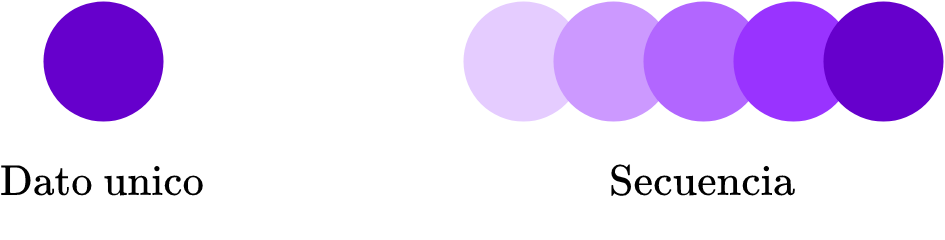
\includegraphics[width=6cm]{images/state-of-art/rnn/ball.png}
    \caption{Ejemplo gráfico de un dato único vs. una secuencia.}
    \label{fig:basic_network}
\end{figure}

De esta forma se puede ver la importancia de tener información temporal y como esta se puede usar para resolver predicciones. La información secuencial está presente en el mundo de diferentes formas: audio (secuencia de bits), texto(secuencia de caracteres o de palabras) o valores que se modifican a lo largo del tiempo.
\newline

La forma en que las \acrshort{rnn} funcionan es gracias a un concepto que se conoce como memoria secuencial. La memoria secuencial es la capacidad para reproducir secuencias de palabras, números, letras, símbolos… de un humano. Por esa razón, es fácil de decir el abecedario y, sin embargo, es más difícil decir el abecedario hacia atrás.
\newline

Usando algún tipo de bucle dentro de la red se puede emular esta memoria secuencial para que una arquitectura de red pueda usar información previa y así poder procesar el cálculo de un nuevo valor. Esta información que es traspasada usando el bucle es lo que se conoce como estado oculto ($h$, \textit{hidden state} en inglés) y contiene información de los valores de entrada previos.
\newline

Cuando se hace referencia a una \acrshort{rnn}, se está hablado de una red que al menos una de las capas es recurrente y por lo tanto tiene algún tipo de bucle. Es decir, pueden existir una \acrshort{rnn} con una sola capa recurrente o bien una \acrshort{rnn} con dos capas recurrentes o cualquier tipo de combinación con al menos una capa recurrente. Se muestra a continuación varios ejemplos:
\begin{figure}[H]
    \centering
    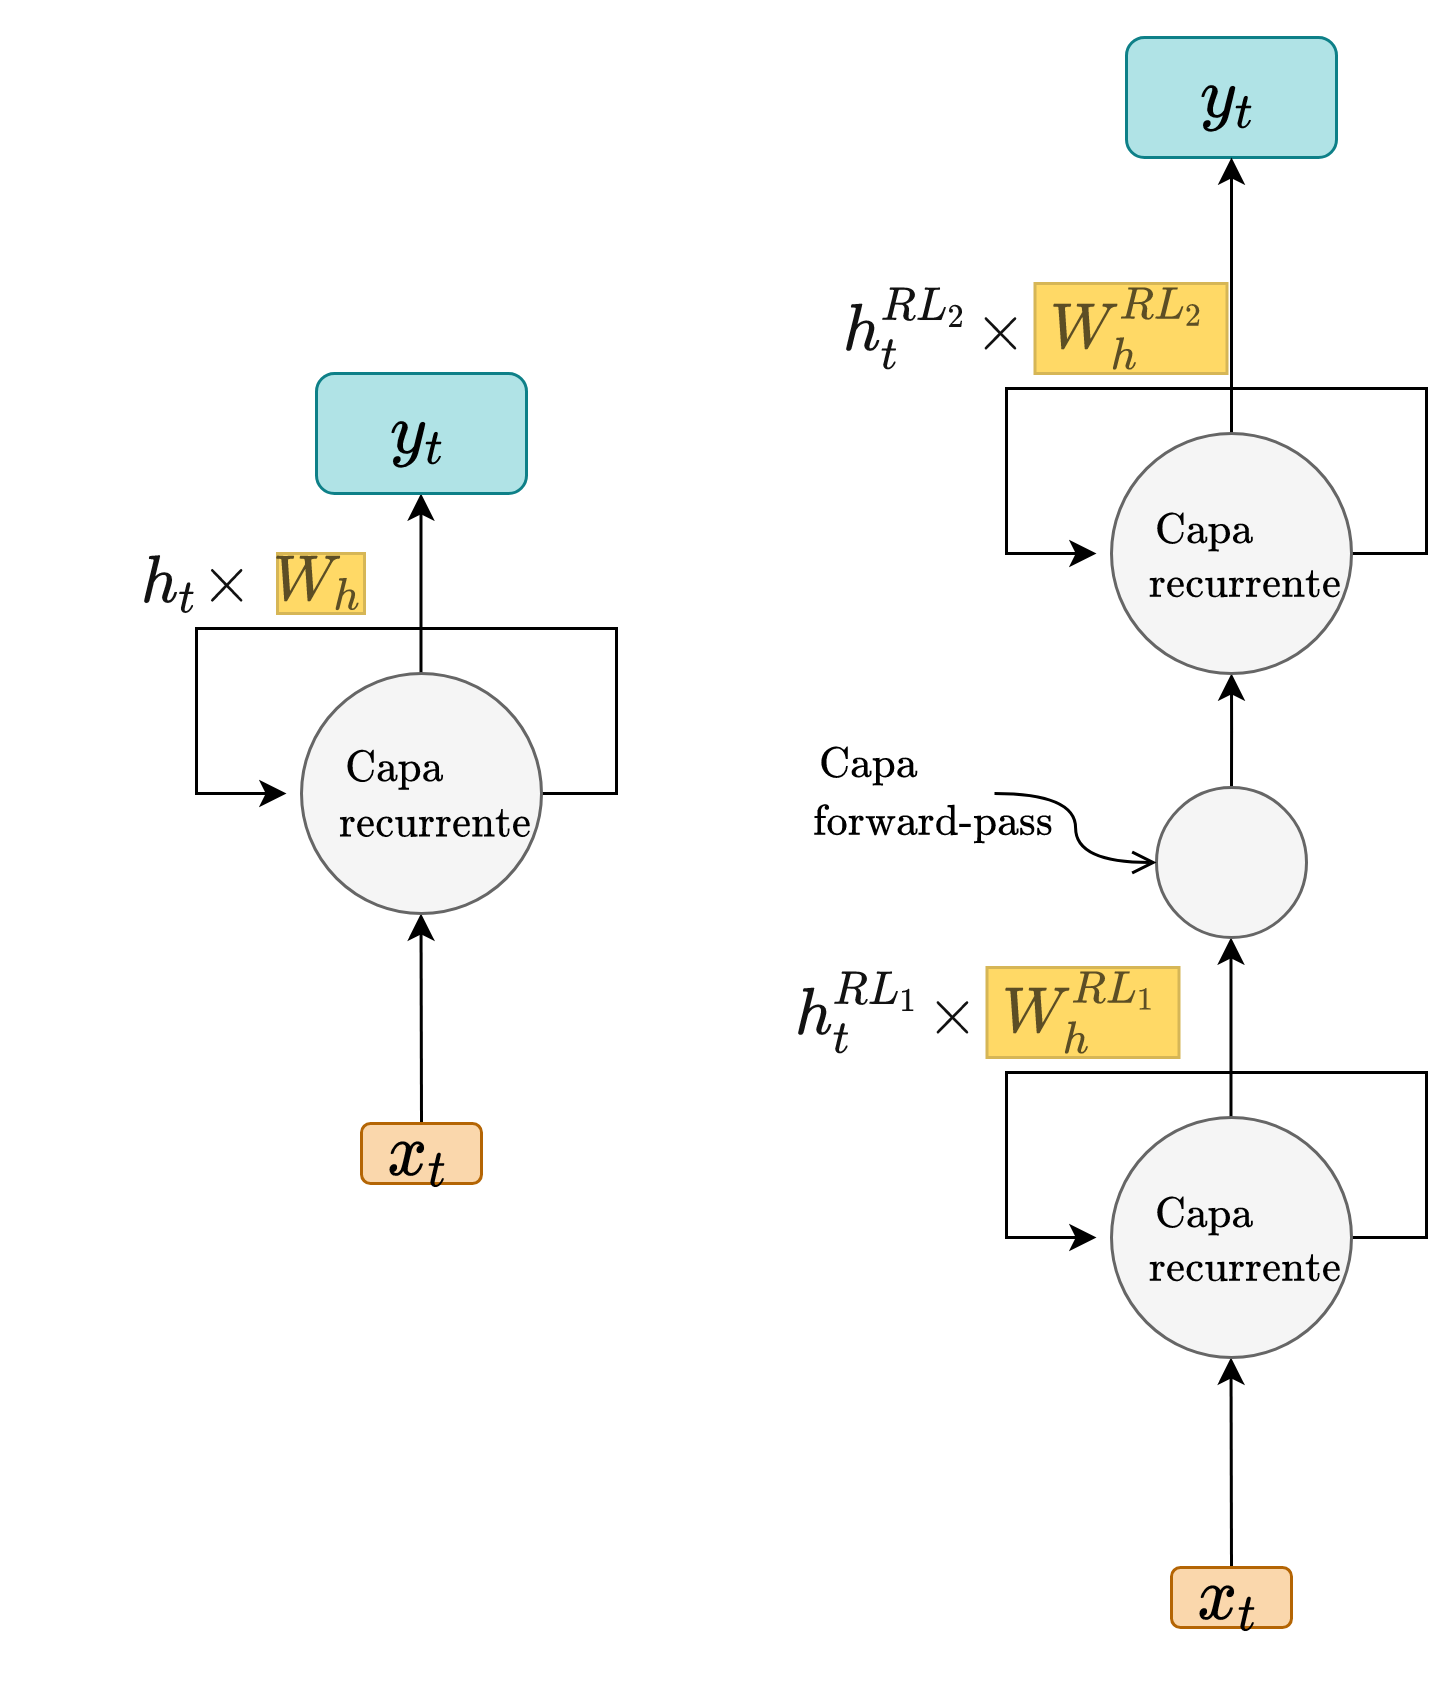
\includegraphics[width=8cm]{images/state-of-art/rnn/rnn-compact.png}
    \caption{Varios ejemplos de \acrshort{rnn}}
    \label{fig:rnn-compact}
\end{figure}

A partir de ahora, en vez de representar el bucle con una conexión reflexiva, se hará usando el eje horizontal para cada una de las iteración y de forma que queda una cadena de redes enlazada. Esta es la forma más común de ver las \acrshort{rnn} representadas.
\newline

En el anterior diagrama, se ha introducido una nueva matriz: $W_h$. Esta matriz es la matriz propia de pesos para el vector $h$. Además, como puede haber varias capas recurrentes, para diferenciar $W_h$ y $h$ se usará el índice $RL_i$ siendo i el número de la capa recurrente.